
We implement our software module in Java and run it on the Android platform.
The software module can be used to generate 
inputs to other applications that capture
driving behaviors and/or road conditions.
To evaluate the convergence time and the accuracy of our 
software module, we developed an offline trace replay engine.
The replay engine sorts the sensor data
based on timestamps, and feeds them into an event listener function in chronological order. 
We use an abstraction called \emph{Trace} to represent the sensor data, 
GPS data and OBD data.
It is similar to SensorEvent used by Android API \cite{sensor}
but provides more flexibility to store OBD and GPS data. 
The event listener function process each \emph{Trace} 
and process them by sensor type correspondingly. 
The coordinate alignment and linear acceleration estimation logic of
the event listener function are the same
as the software module on the Android platform.
The trace replay engine is used to test and evaluate 
the performance of the software module with the traces we collected
by a customized Android app.  
We use the Android app collected more than 10,000 miles
driving data over the last two years. 
We mount Xoom tablet in the bag of the passenger seat and 
use power on/off as indicator to start/stop the app. 


\subsection{Evaluation Settings}

We primarily evaluate the performance of our software module in two aspects, 
i.e., convergence time and linear acceleration estimation accuracy.
We use our trace replay engine to replay the trips collected 
from 13 different drivers over the last two years.
We conducted comparative experiments to evaluate the performance
of the following two approaches:
\begin{itemize}
\item[*]
\textbf{Slope-Aware}: The software module we proposed that includes selective training
and linear acceleration estimation. 
\item[*] \textbf{State of the Art}:
We used the algorithm proposed in \cite{wang2013sensing}, 
the approach is discussed in Section \ref{section_alignment}. 

\end{itemize}


\subsection{Dataset Statistics}

\begin{figure}[!tbph]
	\begin{center}
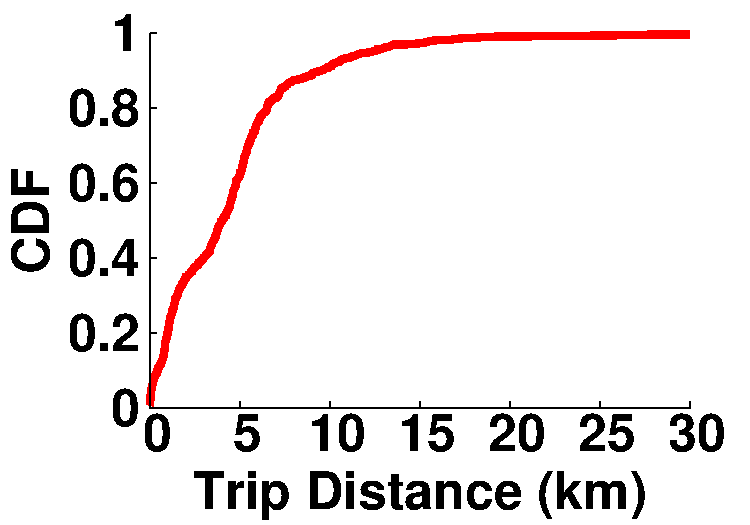
\includegraphics[width=2.1in,angle=0]{Figs/SlopeAware/all_dist.pdf}
\hspace{-0.6cm}
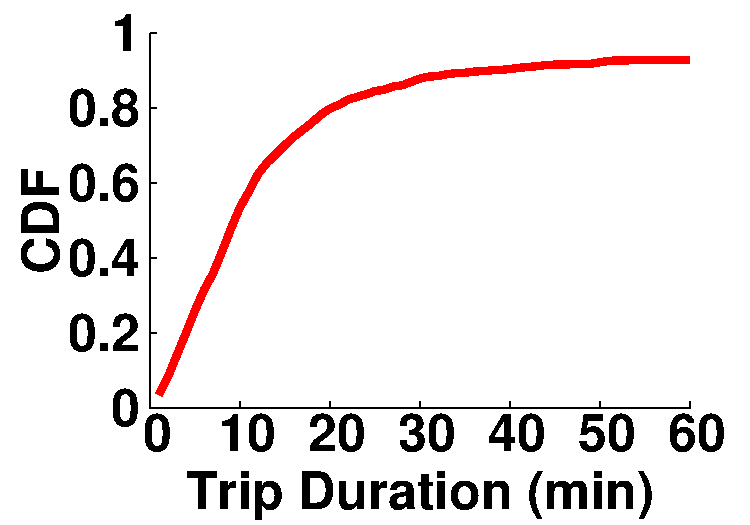
\includegraphics[width=2.1in,angle=0]{Figs/SlopeAware/all_time.pdf}
\hspace{-0.5cm}
\vspace{-0.0cm}
\caption{More than $80\%$ of urban trips have a driving distance less than $7km$.
And more than $80\%$ of the trips have a duration less than $15mins$.}
\vspace{0.0cm}
\label{tripstats}
\end{center}
\end{figure}


To evaluate our slope-aware linear acceleration estimation module, 
we compare it with the accelerations calculated from OBD speeding
data. 
We collected OBD and sensor data from 13 different drivers. 
The dataset covers 5,000 miles in urban area and 5,000 miles on the highway. 
One important feature our software module provides is the fast convergence
time on coordinate alignment under sloping roads.
This feature enables real-time applications like hard 
brake warning similar to Snapshot \cite{snapshot} 
but requires no additional hardware. 
Firstly, we examine the distance and duration of each trip.
The statistics of 904 urban trips are summarized in Fig. \ref{tripstats}.  
As can be seen from the figure, most of the trips have a duration less than $20min$.
This is common for working professionals and students who are 
driving between home and office.
Given short trips like these, it is critical to develop
a fast alignment algorithm to enable real-time applications.


\subsection{Coordinate Alignment Convergence Time}

\begin{figure}[!htbp]
\begin{center}
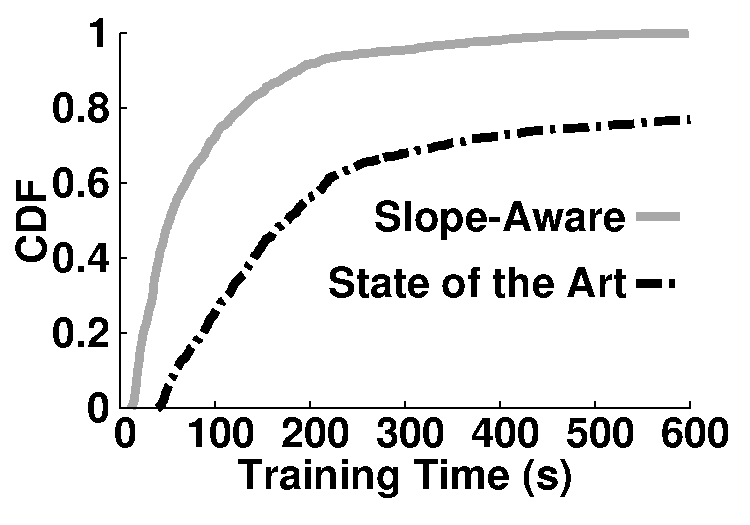
\includegraphics[width=2.8in,angle=0]{Figs/SlopeAware/alignment.pdf}
\vspace{0.0cm}
\caption{The training or convergence time used for coordinate alignment.}
\label{alignmenttime}
\vspace{-0.2cm}
\end{center}
\end{figure}

The convergence time of a coordinate alignment algorithm is critical
for real-time applications such as hard brake warning \cite{snapshot}. 
To evaluate the convergence time, we extract the straight road driving segments and fed them into the replay engine.
The engine stops when the accuracy of coordinate alignment is within
a predefined percentage of the accuracy when we use the segments of the entire trip to train.
As shown in Fig. \ref{alignmenttime}, 
there is a substantial improvement on the convergence speed.
Slope-aware solution can converge in less than $2min$ in more than
$80\%$ of the cases, 
while it takes much longer time to train the rotation matrix if
the algorithm does not consider slope caused deviations.
The convergence time heavily depends on road conditions. 
For the trips with level roads and fewer bumps, it generally
takes less time to converge.
On the other hand, for the trips with lots of slopes and bumps on the road, 
it takes much longer time to converge due to less training opportunities.


\subsection{Linear Acceleration Estimation Accuracy}

\begin{figure}[!htbp]
\begin{center}
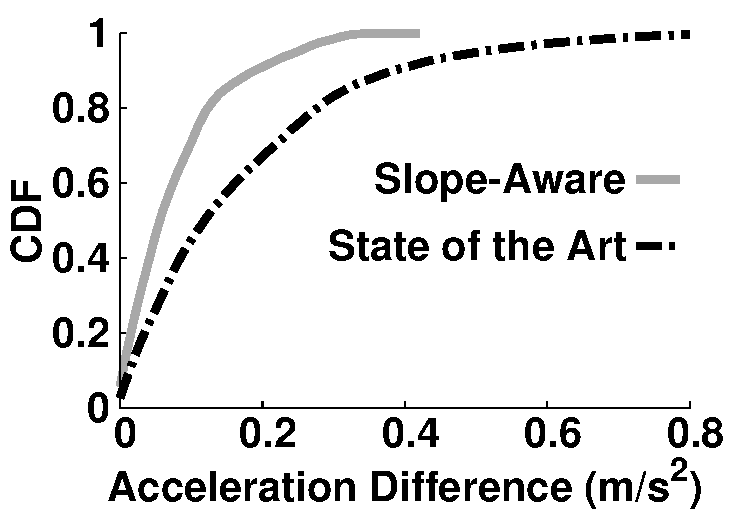
\includegraphics[width=2.8in,angle=0]{Figs/SlopeAware/accdifference.pdf}
\vspace{0.0cm}
\caption{The difference between estimated linear acceleration and ground truth. 
The ground truth is the acceleration calculated by OBD speeding data.}
\label{accdifference}
\vspace{-0.2cm}
\end{center}
\end{figure}


To capture driving behaviors such as brakes and accelerations, 
we are interested in the linear acceleration along the heading
direction of the car. 
Aligned accelerometer cannot be used directly for this purpose
due to the sensed gravitational force component when the car is 
driving on a slope, which leads to vehicular acceleration 
overestimation or underestimation and causes false negatives/positives
on brake/acceleration reports. 

In our evaluation, we compare the estimated accelerations with the calculated
accelerations. 
For slope-aware linear acceleration estimation, we train the rotation matrix
until it converges and deduct the gravitational force components based
on our slope estimation method.
As can be seen from Fig. \ref{accdifference}, the slope-aware solution
has less than $0.2m/s^2$ difference in more than $90\%$ of the cases. 
Comparing with the state of the art, the slope-aware solution is 2 times 
more accurate. 
Also, slope-aware solution limits the linear 
acceleration estimation error to be around $0.4m/s^2$.
The large error of slope unaware solution comes from misalignment
and the lack of slope estimation. 

 
